\documentclass[10pt,letterpaper]{article}

\usepackage{cogsci}
\usepackage{pslatex}
\usepackage[nodoi]{apacite}
\usepackage{graphicx}
\usepackage[american]{babel}
\usepackage{amsmath}
\usepackage[section]{placeins}
\usepackage{enumitem}

\title{Children's Online Processing of Ad-Hoc Implicatures}
 
\author{{\large \bf Erica J. Yoon} \\
  \texttt{ejyoon@stanford.edu} \\
  Department of Psychology \\
  Stanford University
  \And {\large \bf Yunan Charles Wu} \\
  \texttt{ywu15@wabash.edu} \\
  Department of Psychology \\
  Wabash College
  \And {\large \bf Michael C. Frank} \\
  \texttt{mcfrank@stanford.edu} \\
  Department of Psychology \\
  Stanford University}


\begin{document}

\maketitle

\begin{abstract}
Language comprehenders routinely make pragmatic inferences that go beyond the literal meanings of utterances. If A said ``I ate some of the cookies,'' B should infer that A ate some \emph{but not all}. Children perform poorly on experimental tests of scalar implicatures like this, despite their early-emerging sensitivity to pragmatic cues. Our current work explores potential factors responsible for children's successes and failures in computing pragmatic inferences. In two experiments, we used an eye-tracking paradigm to test children's ability to compute implicatures when they have access to contextual alternatives to the target word (Experiment 1), and when they hear prosodic cues that emphasize the contrast between the target and alternative (Experiment 2). We found that by the time children are four years old, they successfully identify the inferential target referent in this paradigm; with supportive prosodic cues, we saw evidence of success in three-year-olds as well. In sum, with sufficient contextual support, preschool children are capable of making online pragmatic inferences.

\textbf{Keywords:} 
Pragmatics; implicature; eye-tracking; cognitive development

\end{abstract}

\section{Introduction}

Language comprehension involves not only interpreting the literal meanings of words in utterances, but also understanding the communicative intentions behind what is said. Listeners make \emph{pragmatic implicatures}, inferences about speakers' intended meanings that go beyond the semantics of their utterances \cite{grice1975logic}. One common type of implicatures, called  \emph{scalar implicatures}, involves scales built based on the knowledge of \emph{lexical} alternatives \cite{horn1972}. For example, if A says to B, ``Some of the students failed the test,'' B may infer that A intended to say ``Some, \emph{but not all}, of the students failed the test.'' That is, A's use of the term ``some'' implicates that the stronger scalar alternative ``all'' is negated. 

Whereas adults readily compute scalar implicatures (\emph{SI}s), children tend to perform poorly on SI tasks (e.g., \citeNP{noveck2001children, papafragou2003scalar, huang2009semantic}). For example, given a context in which three out of three horses jumped over a fence, adults reject a statement such as ``some of the horses jumped over the fence'' as infelicitous, whereas children typically judge it to be acceptable \cite{papafragou2003scalar}. 

Children's failures on SI computation are surprising, given their early-emerging sensitivity to the informativeness of utterances. For example, by around approximately five years, children adjust informativeness of their own expressions depending on the listeners' knowledge \cite{matthews2006effect}; reward speakers based on their informativeness \cite{katsos2011pragmatic}; and provide more information when disambiguation between potential referents is difficult \cite{matthews2012two}. Given this body of research, it seems unlikely that children's lack of pragmatic ability per se causes their failures on SI tasks. What then causes children's failures, and what factors can help them succeed on implicature tasks? The current work investigates two potential factors: availability of alternatives to the current term, and cues that highlight the contrast between current term and its alternatives.

On standard accounts, implicature involves generating and negating stronger alternatives to a given term. Upon hearing ``some,'' the listener needs to generate a stronger alternative (``all'') based on lexical knowledge, and then negate it. One potential cause of children's difficulty with previous SI tasks could be issues generating these alternative terms \cite{barner2011accessing}. If this hypothesis is true, children might succeed on implicature computation if given access to alternatives in the context.

Indeed, there is evidence that children can compute \emph{ad-hoc} implicatures, which depend on contextually- rather than lexically-derived scales \cite{stillerLLD}\footnote{These inferences are sometimes known in the pragmatics literature as ``particularized implicatures,'' in contrast to ``generalized'' implicatures. Here we use the term ``ad-hoc'' implicature as a descriptive term and remain agnostic with respect to the reality of this distinction.}. Children saw three faces, one wearing glasses and a top-hat, one wearing glasses only, and one with no item. When children heard: ``My friend has glasses,'' 3.5-year-old children and older chose the face with glasses only as the referent above chance, successfully computing the implicature ``My friend has glasses, \emph{but not a top-hat},'' given the contextual access to the stronger alternative (face with glasses and top-hat). In our current work we adopt a similar ad-hoc implicature paradigm for eye-tracking, to ask both about factors underlying the previously-observed developmental trajectory and about the decision-making processes underlying children's implicature computation. 

Eye-tracking offers several advantages over purely behavioral measures for examining pragmatic inference. First, it is possible to track participants' gaze as an utterance is being produced, providing moment-by-moment data about responses to spoken language. Second, eye gaze reflects a more implicit measure of comprehension and hence allows for more direct developmental comparisons compared with behavioral choices that may reflect conscious deliberation. 

A previous eye-tracking paradigm looking at SI computation in children \cite{huang2009semantic} suggested that children do not calculate SI during online language processing. For example, when they saw a girl who has two out of four (some but not all) of the socks and another girl who has three out of three (all) of the soccer balls, and heard ``... the girl who has \emph{some} of the soc...,'' unlike adults, children did not look more toward the girl with socks until they heard the disambiguating word ``socks.'' Children might have struggled with SI computation from the lack of access to lexical scales (some-all), and the time constraint to process implicatures (in less than one second). Our current work uses a similar but simpler paradigm that tests children's inference of implicatures given scales that are set up contextually.

Thus, in addition to replicating previous research on ad-hoc implicatures in the online processing context, we are able to pursue two goals: measure the time-course of ad-hoc pragmatic inference; and identify potential factors that contribute to the developmental differences in implicature computation performance. In Experiment 1, we measure implicature performance across a wide developmental range; in Experiment 2, we examine the contribution of contrastive intonation on performance for a subset of age groups. Our findings suggest that young children are able to spontaneously generate implicature inferences when contextual support is present, even though these inferences are slower and harder to make than interpretations of semantically unambiguous utterances.

\section{Experiment 1}

\subsection{Method}

\subsubsection{Participants}

Parents and their 2- to 5-year-old children visiting Children's Discovery Museum in San Jose, CA, were invited to participate in a short video study. The current sample comprised of children who were exposed to English at least 75\% of the time as indicated by their parents. In addition, individual trials with more than 50\% missing gaze data were excluded from analysis, and only participants who completed at least half of the trials according to this criterion were included in the analysis. These exclusion criteria led to a final sample of 108 (out of 113 participants): 24 2-year-olds (M = 2:6, range 2;1--2;11, 10 girls), 28 3-year-olds (M = 3;5, range 3;1--3;11, 19 girls), 24 4-year-olds (M = 4;6, range 4;1--4;11, 13 girls), 32 5-year-olds (M = 5;4, range 5;1--5;9, 9 girls). Children were given a sticker for participating in the study. We also tested fourteen adult participants, undergraduate students recruited through Stanford Psychology credit pool. 

\subsubsection{Stimuli and Design}

On each trial, participants saw two images: a target and distractor, which could either be an item with a single feature (e.g., a plate with only a carrot or only a banana), or an item with double features (e.g., a plate with a carrot and a banana). Each trial contained three phases: in the initial phase (8.5 seconds), two images were presented in silence for two seconds, then a pre-recorded voice said a sentence (e.g., ``Look at these plates. Elmo's plate has a carrot.''). Then, in the anticipatory phase (1.5 seconds), a chime sound played to induce participants' anticipatory gaze. In the following feedback phase (1.5 seconds), a character appeared next to the target with an amusing sound effect. This outcome served to keep the task engaging for participants.

There were three types of test trials (pictured in Figure \ref{fig:age}, bottom). In \emph{inference} trials, the target item had a single feature (e.g., a carrot), and the distractor item had two features, one that was common with the target (e.g., a carrot) and the other feature that was unique (e.g., a banana). The test sentence named the feature that was common to the target and distractor. Thus, if participants understood that ``Elmo's plate has a carrot'' implicates ``Elmo's plate has a carrot \emph{but not a banana},'' given the context, they should look more toward the target than the distractor, but otherwise look equally to both.

There were two additional trial types, with semantically unambiguous targets: \emph{Control-double} trials looked identical to inference trials, but the target and distractor were switched, such that the double-feature item was the target and the single-feature item was the distractor, and the test sentence named the unique feature on the target. \emph{Control-single} trials presented two items that each had a unique single feature, and either could be the target. Children saw 4 inference, 4 control-double, and 4 control-single trials; adults saw 6 inference, 6 control-double, and 12 control-single trials. 

There were six sets of item and feature types, and the features were named with nouns found on the  MacArthur-Bates Communicative Development Inventory word list \cite{fenson1994variability}. Two orders of the test trials were created, such that trial types and item types were counterbalanced and trial order was pseudo-randomized across the two orders.

\subsubsection{Procedure}


\begin{figure*}[t]
\begin{center} 
  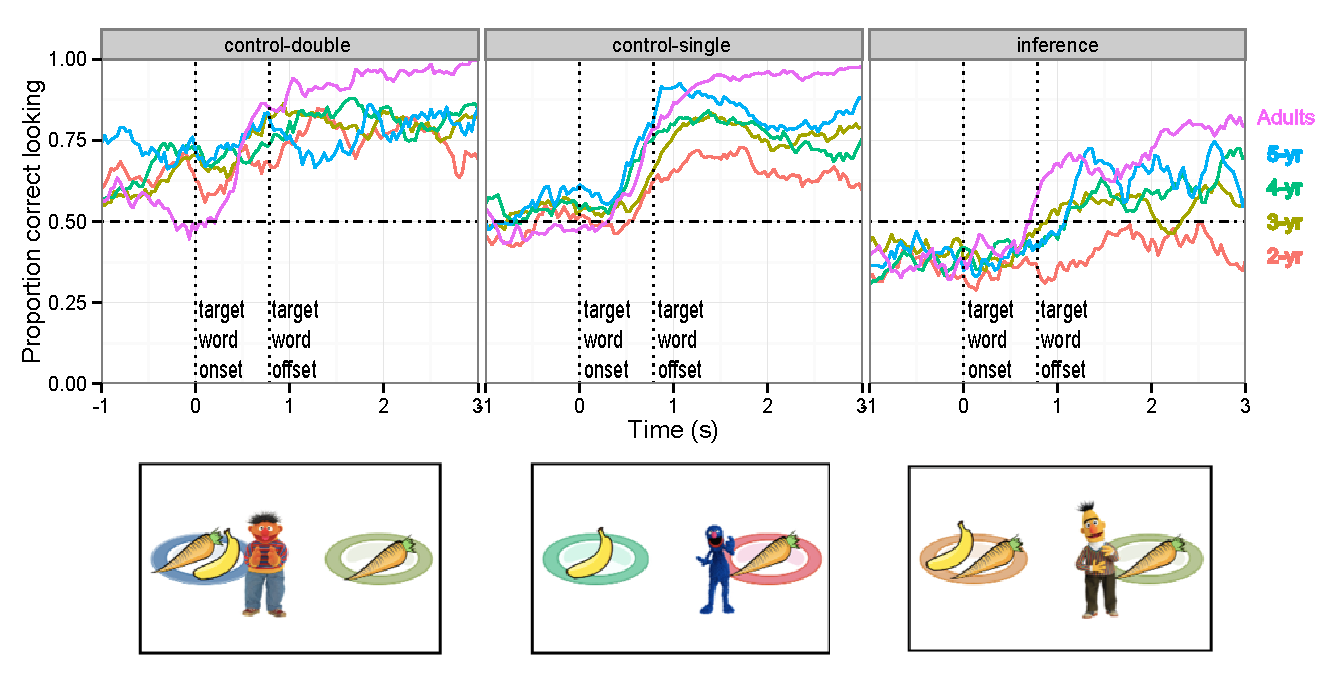
\includegraphics[width=.9\textwidth]{figures/expt1-accuracy.pdf}
  \caption{\label{fig:age} Proportion of 2- to 5-year-old children and adults looking to the target image as the utterance unfolds. Time 0 represents the target word onset. Proportion correct looking is defined by looks to the target divided by the total looks to both the target and the distractor. Bottom panels show example stimuli from each condition; the named character emerged at the end of the trial to mark the correct target.}
  \end{center} 
\end{figure*}

Participants sat in a booster seat, approx. 60 cm away from the monitor of an SMI RED 120 Hz binocular remote eye-tracker. Participants were introduced to the task as watching a short video. The video began with a short Elmo video clip that lasted for 1-2 minutes, during which any necessary adjustments to the eye-tracker and participants' chair positions were made. The eye-tracker was then calibrated using a 2-point calibration and validation of the calibration points. Then participants were introduced to Sesame Street characters and told `Today, [they] will show us lots of fun things. Are you ready? Let's go!' Following the introduction, participants saw two gaze-contingent practice trials, with unambiguous targets that differed from the test items. Then children watched 16 test trials and adults watched 24 test trials, as well as 4 filler photos of children playing and 2 Elmo video clips, presented at a pseudo-random points between test trials. The video lasted approximately 8 minutes.

\subsection{Results and Discussion}

Participants of all ages looked to the targets in both control-double and control-single trials reliably above chance (50\%; Figure \ref{fig:age}). There were age differences in the speed of looking at the target and the proportion of correct looking across both control trial types.

For inference trials, children of 4 years and above robustly looked to inferential targets (for 4-year-olds: $t(23) = 2.74$, $p =.01$). For example, upon hearing ``Bert's plate has a carrot,'' older children identified the plate with only a carrot as the referent rather than the plate with a carrot and a banana, replicating \citeA{stillerLLD}'s findings of ad-hoc implicature (though that study found successes in 3.5--4-year-old children as well). Although previous studies are not directly comparable due to low-level differences in the task and materials, our finding is consistent with the hypothesis that children's inferential ability might have been obscured in previous SI tasks due to the unavailability of lexical alternatives (e.g. ``all'' given ``some''; \citeNP{barner2011accessing}).

We additionally observed an unpredicted trend in two-year-olds' behavior: they did not disengage from distractors relative to their baseline bias prior to hearing the target word, and were marginally \emph{below} chance in their overall performance ($t(23)  = 1.93$, $p = .07$). We return to this pattern in the General Discussion and speculate about the sources for the observed developmental changes.

We fit a linear mixed-effects model\footnote{All mixed-effects models were run using the \texttt{lme4} package, version 1.1-7. The random effects structure for this model was as follows: \texttt{(trial type $|$ subid) + (age + trial type $|$ item)}.} to measure the effects of trial type and age on the proportion of children looking to the target between 1 and 4s after noun onset (Table \ref{tab:lmer1}). We selected this time window because participants would have to wait until the end of target noun (0.8 seconds on average) to know they should switch to the inferential target, given the absence of a disambiguating continuation (e.g., ``Elmo's plate has a carrot \emph{and banana}.''). Results of the mixed-effects model indicate significant main effects of trial type and age: participants looked to the target significantly less in inference trials compared to control-single trials, and across all trial types, participants' looking to target increased with age. 

\begin{table}[t]
\caption{\label{tab:lmer1}  Coefficient estimates from mixed-effects models predicting proportion of looks to target in Experiment 1.} 
\begin{center} 
\begin{tabular}{l r r r l} 
\hline
Predictor  &  Value (SE) & \emph{t}-value\\
\hline
Intercept (Control-single)  & .60 (.05) & 12.22 \\
Age & .04 (.01) &  3.21 \\
Control-double & .10 (.06) & 1.78 \\
Inference & -.24 (.07) & -3.69 \\
Age $\times$ Control-double & -.02 (.01) & -1.17 \\
Age $\times$ Inference & .01 (.02) & .87 \\
\hline
\end{tabular} 
\end{center} 
\end{table}

We next analyzed participants' reaction times \cite{fernald2008looking}. We selected trials on which participants were looking at the distractor at the point of disambiguation, and measured the average length of time prior to a shift to the target. Looks to the target were slower in inference trials compared to both control trial types across all age groups (Figure \ref{fig:rt}). We next fit a linear mixed-effects model with the same structure as the previous analysis, but predicting reaction time rather than accuracy. This model again showed significant main effects of trial type ($\beta = .109$, $p <.001$) and age ($\beta = .341$, $p <.001$) on the average RT, with no interaction (largest $\beta = .02$, $p >.24$). Inference trials were generally slower compared to unambiguous control trials, regardless of the participants' age. 

\begin{figure}
\begin{centering} 
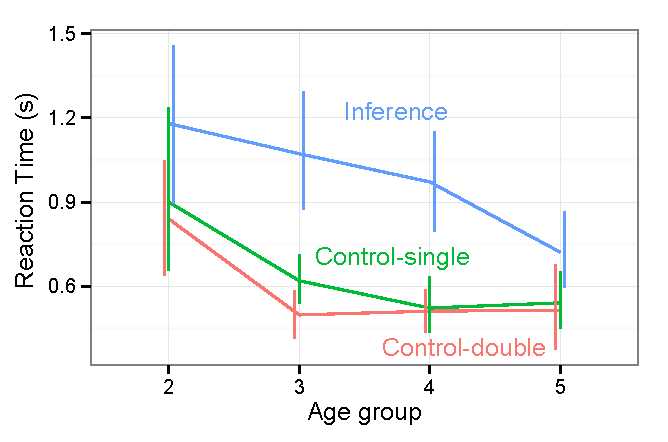
\includegraphics[width=3.2in]{figures/expt1-rt.pdf}
\caption{\label{fig:rt} Average reaction times for first switches to target in trials in which participants were looking at the distractor (and not the target) at the target word onset. Error bars indicate 95\% confidence intervals.}
\end{centering} 
\end{figure}

\section{Experiment 2}

In Experiment 1, we found that 4- and 5-year-olds looked more at the target of simple ad-hoc implicatures, but younger children did not show the same effect. In Experiment 2, we explored whether prosodic stress could improve children's performance. Contrastive stress---a change in pitch, characterized by an initial drop followed by a rise---is a signal of the contrast between possible referents and can facilitate processing of simple references for adults \cite{ito2008anticipatory}.

For children, evidence of the use of contrastive stress is more mixed \cite{cutler1987}. Two recent papers found evidence for sensitivity to contrastive stress in 6-year-olds \cite{sekerina2012,ito2012}, but both of these studies found that processing was relatively slow and only present in cases where contrast was highly supported by the discourse context. On the other hand, \citeA{kurumada2014} found that younger preschoolers could make use of contrastive stress on a simple forced-choice task. Children saw a picture of a zebra and a picture of an okapi (an animal that resembles a zebra); when they heard ``It LOOKS like a zebra'' with contrastive stress on the word ``looks,'' children reliably chose the picture of the okapi, if they heard the same speaker use simpler sentences (e.g., ``It's a zebra'') to refer to unambiguous targets. Thus, the evidence is mixed on whether preschoolers are sensitive to contrastive focus as a cue for reference resolution. 

In the current experiment, we investigate whether a contrastive stress on the final noun (e.g., ``Elmo's plate has a CARROT'') in the inference trials would assist children in identifying the pragmatically-correct referent.

\subsection{Method}


\begin{figure*}[t]
	\center{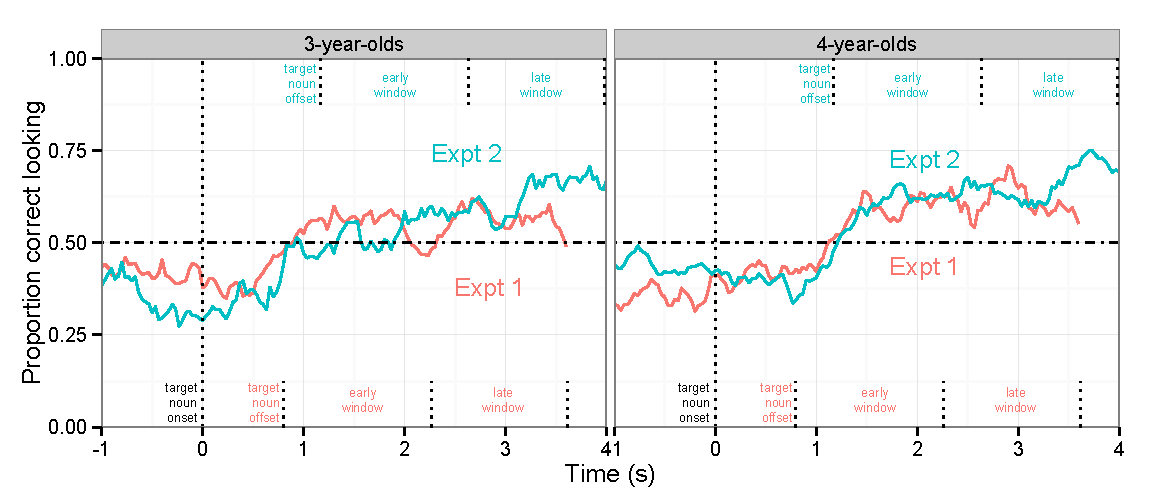
\includegraphics[width=.8\textwidth]{figures/expt12-accuracy_overTime.pdf}}
	\caption{\label{fig:pros0} Proportion of 3- and 4-year-old children looking to the target image as the utterance unfolds, comparing across two Experiments. Early window is the first half of the period between offset and end of trial for each Experiment, and late window is the second half.}
\end{figure*}

\subsubsection{Participants}

Participants were recruited as in Experiment 1. For Experiment 2, we focused on 3- and 4-year-olds. Out of 57 initial participants, the final sample was chosen based on the same criteria as Experiment 1, and consisted of 17 3-year-olds (8 girls), and 31 4-year-olds (18 girls).

\subsubsection{Stimuli, Design, and Procedure}

The stimuli, design and procedure were identical to Experiment 1, except for one change: Target nouns in inference trials were produced with contrastive stress (low-high-low pitch accent and longer duration, 1.2 seconds on average). Based on previous findings that children identify contrastive prosody based on the norms set within an experiment \cite{kurumada2014}, we included prosodic cues only on inference trials. 

\subsection{Results and Discussion}

A linear mixed-effects model predicting accuracy based on age and trial type in Experiment 2, as in Experiment 1, showed a significant main effect of trial type ($\beta = -.216$, $p <.001$), such that looking at target was lower in inference trials than in control trials. There was no significant main effect of age or interaction between age and trial type (largest $\beta = .05$, $p >.18$), though t-tests indicated that 4-year-olds looked reliably more than chance to inferential targets ($t(30) = 5.34$, $p <.001$), while 3-year-olds did not ($t(16) = 1.60$, $p =.13$). A linear mixed-effects model looking at the reaction times of making first switch from distractors to targets as in Experiment 1, found a significant main effect of trial type ($\beta = .109$, $p <.001$) on the average RT, with no interaction ($\beta = .369$, $p <.003$). Thus, looking at inferential targets was slower and overall lower compared to unambiguous targets, but was above chance (for 4-year-olds), consistent with what was observed in Experiment 1.

To determine the effect of prosodic cues on children's inferential processing, we compared looking at targets across both Experiment 1 and 2 for inference trials (Figure \ref{fig:pros0}). Children's looking toward inferential targets increased slightly Experiment 2, especially towards the end of trials. We conducted a post-hoc analysis in which we split trials into an early and late period (Figure \ref{fig:0prosbar}). In the late window, both 3- and 4-year-olds looked at the correct inferential target above chance for Experiment 2 (3-year-olds: $t(16) = 2.47$, $p < .03$). In contrast, 3-year-olds in Experiment 1 were not above chance in either window (largest $t(27) = 1.49$, $p = .15$). Nevertheless, these two groups did not differ from one another. We fit a linear mixed-effects model for inference trial accuracy with experiment and age as predictors and did not find any interactions (largest $\beta = .07$, $p > .27$). Thus, although there was a numerical advantage for both age groups in inference trials in Experiment 2, this advantage was not statistically reliable. 

Overall, we found a hint of successful implicature computation for the three-year-olds in Experiment 2, but we interpret this result with caution given the lack of a significant difference between the two experiments. Nevertheless, these findings may suggest some congruence with the results of \citeA{stillerLLD}. In that study, 3.5-year-olds succeeded at above-chance levels in resolving ad-hoc implicatures, but the referring expressions were produced naturalistically by an experimenter and may have contained some contrastive stress on the target noun. 

\begin{figure}[h!]
\begin{center} 
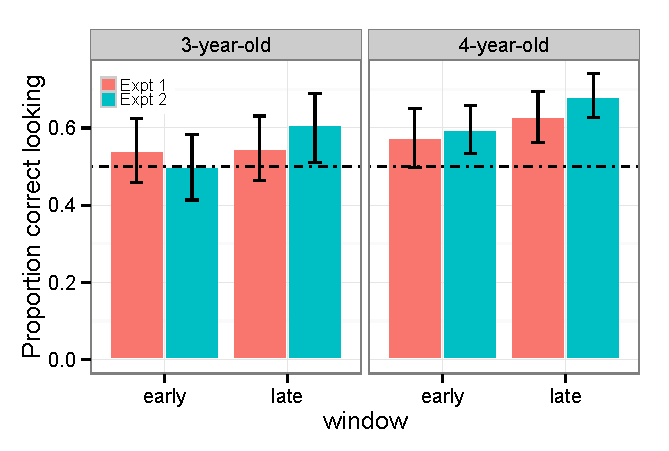
\includegraphics[width=3.2in]{figures/expt12-accuracy_split.pdf}
\caption{\label{fig:0prosbar} Looking to the target as a proportion of looking to the target and distractor in inference trials, averaged during two windows. Error bars indicate 95\% confidence intervals.}
\end{center} 
\end{figure}

\section{General Discussion}

Are young children able to make pragmatic inferences in online language processing? The current work looked at children's understanding of ad-hoc (contextually-based) implicatures using an eye-tracking paradigm, and found that adults and older preschoolers showed robust looking toward inferential targets, although at slower and overall lower rates compared with semantically unambiguous targets. On the other hand, younger children did not show successful implicature computation within the time windows we examined. In a second experiment we found a limited boost in performance for the use of contrastive stress (consistent with other literature on the lack of sensitivity to prosodic cues for preschoolers). Nevertheless, 3-year-olds in this experiment did show some signs of above-chance performance, though they did not differ significantly from 3-year-olds in Experiment 1.  

Our findings are broadly convergent with previous behavioral work on this topic \cite{stillerLLD}, suggesting that the ability to make ad-hoc implicatures is fragile but measurable in 3-year-olds (with contrastive prosody) and more robust with 4-year-olds. Nevertheless, accuracy in the two paradigms differed: The rate of looking to the inferential target was overall lower in the current study than the accuracy rates in \citeA{stillerLLD}, even though the current paradigm was simpler (with two referent choices instead of three). This difference is plausibly due to the difference between eye-tracking and multi-alternative forced-choice paradigms: in particular, accuracy in our paradigm reflects graded patterns of looking across targets rather than a single forced-choice judgment.

One unpredicted and intriguing---albeit tentative---finding was that 2-year-olds not only did not look at the correct inferential target, but seemed to look if anything more toward the distractor. A potential explanation for this pattern comes from the inhibitory demands of our task. The two items in inference trials differed in salience: Since the distractor item contained an extra referent (e.g., a carrot and a banana), it was likely to be more salient. Supporting this idea, looking to the two-referent item was greater than chance during the baseline period of each trial. Perhaps 2- and 3-year-olds had difficulty disengaging from this more salient (and logically possible) distractor item in favor of the inferentially-correct target item. Inhibitory control is difficult for children and continues to develop throughout the period we studied here (e.g.,  \citeNP{davidson2006development}). In addition, several recent studies suggest that inhibitory control might affect word recognition in similar eye-tracking paradigms \cite{yurovskybeyond,nordmeyer2013measuring}. Future work should thus address this possibility by explicitly manipulating the salience of potential pragmatic targets.

Our findings are consistent with previous claims that children's difficulties with SI are caused by their lack of access to linguistic scales (e.g., some-all; \citeNP{barner2011accessing}). Since our paradigm featured pictures of all the possible referents, the demands of generating scalar alternatives were reduced. This aspect of the study also probably led to the relatively faster generation of implicatures than has been found in previous processing studies. It has previously been suggested that children are not able to compute SIs in a timely way during online language comprehension (e.g., \citeNP{huang2009semantic}). The current work suggests another possibility: implicature computation may indeed be delayed compared to interpretations of unambiguous utterances, even for adults. However, with contextual access to scales relevant to implicature computation, children can generate implicatures quickly enough for them to be relevant to ongoing conversation. 

Even young children are sensitive to the communicative intentions behind utterances they hear \cite{clark2009first,baldwin1993early}. Our work adds to the body of evidence suggesting that by preschool age they are able to generate sophisticated pragmatic implicatures as well, even though these inferences are easily masked by other processing demands of specific contexts and situations. Overall, our current work takes one step further towards reconciling children's early-emerging communicative abilities with the complex pattern of successes and failures that they show in Gricean pragmatics.

\section{Acknowledgments}

We thank the parents, children, and staff at the San Jose Children's Discovery Museum. This work was supported by a Postgraduate Scholarship and Doctoral Program Fellowship provided by Natural Sciences and Engineering Research Council of Canada.

\bibliographystyle{apacite}

\setlength{\bibleftmargin}{.125in}
\setlength{\bibindent}{-\bibleftmargin}

\bibliography{YoonCogSci15}


\end{document}
